\documentclass[12 pt]{article}

\usepackage{amsmath,amstext,amsgen,amsbsy,amsopn,amsfonts,graphicx,
theorem}

\renewcommand{\baselinestretch}{1.0}

\begin{document}

\title{A Review of Return Maps for R\"ossler and the Complex Lorenz}
\author{Keith M. Carroll\\ School of Physics \\ Georgia Institute of Technolology \\ Atlanta, GA}
\date{May 1, 2012}
\maketitle
At first glance, finding and labelling periodic orbits in a chaotic system appears a daunting task.  It even seems unlikely that out the chaotic trajectories in a strange attractor there would even exist periodic orbits and trajectories.  With the clever use of Poincar\'e sections and return maps, there is a methodology to the madness.  Poincar\'e maps not only provide intuition about how the dynamics act but also when properly used, translate into a return map.  The purpose of this work is to review the methods of computing return maps and periodic solutions for the R\"ossler system and to apply this knowledge to the Complex Lorenz equations.  The main difference between the Complex Lorenz and R\"ossler equations is the Complex Lorenz exhibit symmetries.  To overcome this obstacle, we review symmetry reduction methods and apply them to the Complex Lorenz.  Once symmetry is reduced, the Complex Lorenz problem becomes the same as the R\"ossler, and we can use the same methods developed there.  Our first goal, however, is to review how to compute periodic orbits for the R\"ossler system.

\section{R\"ossler System and Return Map}
\label{sec:Ross}
The R\"ossler equations:
\begin{equation}
\begin{split}
  \dot x &= -y -z \\
  \dot y &= x + a y \\
  \dot z &= b + z (x - c) \,,
  \label{eq:Rossler}
\end{split}
\end{equation}
were developed to study chaos as a variant on a harmonic oscillator \cite{CB}.  We start with this system because unlike higher dimensional problems, the full state space can be visualized.  With this in mind, we begin our tour of the R\"ossler system.
For this work, we will focus on parameters given by $a = b = 0.2$ and $c = 5.7$; under these conditions the equilibria are given as:
\begin{equation}
\begin{split}
x_{eq}^{-} &= (\frac{c+D}{2}, -\frac{c+D}{2a}, \frac{c+D}{2a}) \approx (0.007,-0.035,0.035)\\
x_{eq}^{+} &= (\frac{c-D}{2}, -\frac{c-D}{2a}, \frac{c-D}{2a}) \approx (5.693,-28.465,28.465) \\
D &= \sqrt{c^2-4ab}
\end{split}
\label{eq:RossEq}
\end{equation}
The stability of the near and far equilibrium, $x_{eq}^{-}$ and $x_{eq}^{+}$, is obtained from the eigenvalues of the stability matrix $A_{ij} = \frac{\partial{v_{i}}}{\partial{x_{j}}}$:
\begin{equation}
\begin{split}
x_{eq}^{-} : \quad (\lambda_1^-, \lambda_2^-, \lambda_3^-) \approx (0.097-0.995i, 0.097+0.995i, -5.687) \\
x_{eq}^{+} : \quad (\lambda_1^+, \lambda_2^+, \lambda_3^+) \approx (0.193, -5.428i, 5.428i) \\
\end{split}
\label{eq:RossStab}
\end{equation}
Examining a typical trajectory, such as the one in Figure \ref{fig:RossTraj}a, shows that a trajectory not in the basin of attraction for $x_{eq}^{-}$ will spiral away along the unstable direction of $x_{eq}^{+}$ and wander away.  If it is within the basin, the trajectory spirals away from $x_{eq}^{+}$ towards $x_{eq}^{-}$, and once the trajectory comes close to $x_{eq}^{-}$, it lands on the unstable direction of $x_{eq}^{-}$ and spirals outwards.  When it gets far enough out, the unstable $x_{eq}^{+}$ pushes the dynamics back in towards $x_{eq}^{-}$ and the cycle begins again.  The equilibria split the dynamics into those that diverge away and stay away (wandering set of trajectories) and those that are attracted and stay near the equilibrium close to the origin (the non-wandering set of trajectories) \cite{CB}.  It is not obvious that out of this non-wandering set that there should exists periodic orbits, or trajectories such that:
\begin{equation}
\exists T_p : \quad  x(t+T_p) = x(t) \,.
  \label{eq:PerTraj}
\end{equation}
Our goal is to review and generalize the methods to obtaining these solutions.  Our starting point is one of the most powerful techniques used in dynamics: Poincar\'e sections.  A Poincar\'e section can provide intuition about the nature of dynamics, but more importantly, they can be turned into return maps which lead to our periodic orbits.

At first glance, picking a good Poincar\'e section is more an art than anything else, and what constitutes a good Poincar\'e section can only truly be answered once we have gone through the computation for return maps.  We will return to this concept at the end of this section, but for now, we will follow good judgment and define a good Poincar\'e section as one that captures the local dynamics of interest \cite{CB}.  Using our previous example, we want to capture the dynamics in the attractor for the trajectory in Figure \ref{fig:RossTraj}a.  To capture the interesting dynamics, a good Poincar\'e section will cut the spiralling around the $x_{eq}^{-}$, such as the one suggested in Figure \ref{fig:RossTraj}b.

 \begin{figure}[h]
\centering
a.)  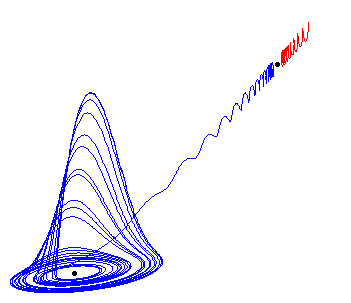
\includegraphics[width=0.35\textwidth]{Figs/Section1/kcRosslerTrajc.png}
b.)
  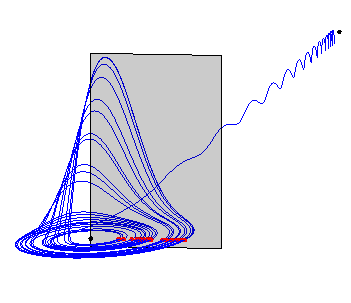
\includegraphics[width=0.35\textwidth]{Figs/Section1/kcRosslerTrajwithPSc.png}
\caption{Trajectories of the R\"ossler system.  The equilibrium $x_{eq}^{-}$ and $x_{eq}^{+}$ are marked in black.  a) A typical trajectory (blue) in the basin of attraction for $x_{eq}^{-}$ spirals towards $x_{eq}^{-}$ and fills out the attractor.  The (red) trajectory shows a typical trajectory that spirals away from $x_{eq}^{+}$.  b) Shows a good Poincar\'e section that will capture the dynamics of interest around $x_{eq}^{-}$.  The section contains the $x_{eq}^{-}$, and as the trajectory crosses the section, each point is marked in red.}
 \label{fig:RossTraj}
\end{figure}

With a good Poincar\'e, we see how the dynamics are governed near $x_{eq}^{-}$; in a typical trajectory such as the one in Figure \ref{fig:RossTraj}b, the trajectories spiral away from $x_{eq}^{-}$ along the unstable manifold and then fold back onto themselves along the stable direction.  To capture all of these dynamics in our Poincar\'e section, we want to start with points that start on the unstable manifold of $x_{eq}^{-}$ \cite{Eth}.  The reasoning for the unstable manifold versus the stable manifold are straightforward: (1) a trajectory placed on the stable manifold will approach the equilibrium, but never quite make it; and (2) the unstable manifold causes the a trajectory to push out, when it comes back in, the contracting nature of $x_{eq}^{-}$ will (almost) place the trajectory back on the unstable manifold to begin the cycle again (Figure \ref{fig:RossUnstable}).
\begin{figure}[h]
\centering
a.)  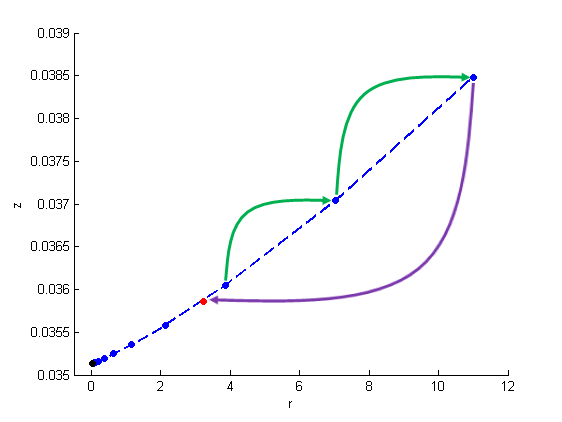
\includegraphics[width=0.35\textwidth]{Figs/Section1/kcsinglettrajectoryalongPSdirection.png}

b.)  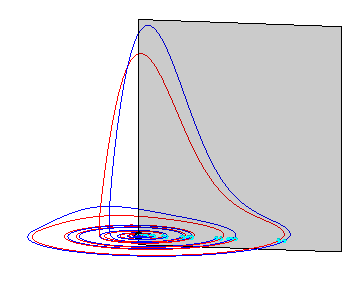
\includegraphics[width=0.35\textwidth]{Figs/Section1/kcRosslerUnstableManPSc.png}
\caption{
 a) Example of the unstable manifold's curve in the Poincar\'e section for a trajectory originating on the manifold.  The equilibrium is marked in black, and the blue points correspond to stretching and the green arrows show directionality.  When the trajectory folds back in (purple arrow) to the turn over point (red), we stop collecting crossings.  Here we have only shown one trajectory marking out a curve, but in practice, one starts with a series of points very close to the equilibrium and along the unstable eigen-direction.
b) Two examples of trajectories that start on the unstable eigen-direction of $x_{eq}^{-}$ (one is in red the other is in blue). As the trajectories fill out the attractor and cross the Poincar\'e section (cyan), they cut out a curve such as the one in part a.
}
 \label{fig:RossUnstable}
\end{figure}

To start on the unstable manifold, we use an initial point for the trajectories very close to $x_{eq}^{-}$ and linear theory dictates the unstable direction and manifold.  As the trajectories evolve with time, the Poincar\'e section marks their $i$th crossings $\hat{x}_i$ until they have fallen back in towards the equilibrium as in Figure \ref{fig:RossUnstable}.  Crossing the Poincar\'e section should only be counted in one direction.  The unstable manifold will carve out a curve as it stretches out in the Poincar\'e section, and as long one fold over is marked, the dynamics of the system will be captured (Figure \ref{fig:RossUnstable}).

To translate this curve into a return map, we invoke the notion of curvilinear distance \cite{SRetMap}:
\begin{equation}
 s_n = \sum_{i = 0}^{n-1} \parallel \hat{x_i} - \hat{x_{i+1}} \parallel
 \label{eq:CurveDis}
\end{equation}
where $\hat{x_i}$ is the position of the trajectory crossing the section and we are summing over all points ordered along the curve originating from the equilibrium $x_0 = x_{eq}^{-}$ to our point of interest $x_n$.  For a given trajectory, we define the next distance along this curve as $s_{n+1}$.

Tracking the curvilinear distance provides the return map: the unstable manifold pushes a trajectory out (distance along the curve increases), at a certain point on this manifold, the trajectories are pulled back in (distance along the curve shrinks).  In other words, the distance tells how a trajectory is pushed out or pulled back in as it spirals around $x_{eq}^{-}$, and this will act as a return map if we look at $s_n$ versus $s_{n+1}$.
\begin{figure}[h]
\centering
  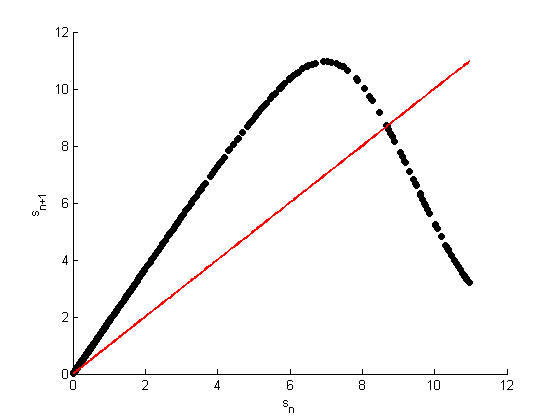
\includegraphics[width=0.35\textwidth]{Figs/Section1/kcrosslerretmap.png}
\caption{
 The return map for the R\"ossler system.  The black marks the return map, and the red shows how to use the return map to find the periodic orbit in Figure \ref{fig:RossPO}.  This a plot of the curvilinear distance $s_n$.  For the high order lengths, the periodic orbits of the R\"ossler system can be found through methods such as the Newton root finding method after iterating the map or with a multi-point Newton method \cite{CB}.
}
 \label{fig:RossRetmap}
\end{figure}

Running this for the R\"ossler system, we arrive at Figure \ref{fig:RossRetmap}.  Using this return map, periodic orbits of length $1$ (spiral around $x_{eq}^{-}$ once) are found by calculating distances such that $s_n = s_{n+1}$.  Return maps can be used to compute cycles of length $k$ by solving those which solve $s_n = s_{n+k}$.  A few simple examples are shown in Figure \ref{fig:RossPO}.

\begin{figure}[h]
\centering
a.)  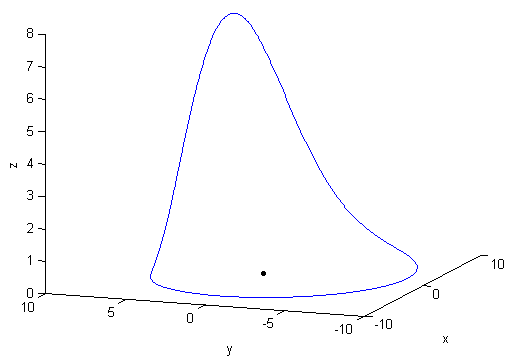
\includegraphics[width=0.35\textwidth]{Figs/Section1/kcross1cyclec.png}
b.)
  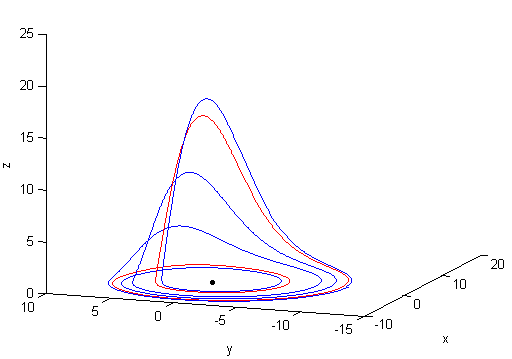
\includegraphics[width=0.35\textwidth]{Figs/Section1/kcross24cyclesc.png}
\caption{a) Cycle $\overline{1}$ for the R\"ossler system. b) Cycles $\overline{01}$ (red) and $\overline{0111}$ (blue).  The meaning of these names for the cycle will be given in section \ref{sec:Retmaps}}
 \label{fig:RossPO}
\end{figure}

We have demonstrated that for a chaotic system, in this case the R\"ossler system, we can find periodic orbits with return maps based on curvilinear distance along the unstable manifold in a section. We mentioned earlier that the choice of a good Poincar\'e section becomes easier to understand once we have gone through the return map calculation.  The Poincar\'e section needs to cut the trajectories in such a way that all the interesting dynamics of the attractor are captured.  Since we are looking at curvilinear distance along the unstable manifold with respect to the attractor, the section should include the equilibrium point near and directly involved with the attractor, but this is not necessarily a requirement that needs to be taken to heart.  One could in principle generalize the theory for sections not containing the equilibrium, but if not careful, certain periodic orbits could be lost.  As a result, it is not a bad idea to make sure the section includes the equilibrium.  There is also some literature which suggests multiple Poincar\'e sections may be necessary \cite{Atl}; however, for our purposes here of finding periodic orbits of the R\"ossler attractor, this section will suffice.
To summarize and generalize what we have done here, we:
\begin{enumerate}
    \item Determined the equilibria and their stable and unstable directions,
    \item Found which equilibria were involved in the attractor,
    \item Chose a Poincar\'e section that captures the dynamics of interest,
    \item Marked how the unstable manifold crossed the section,
    \item Calculated the curvilinear distance along the curve,
    \item Turned the curvilinear distance into a meaningful return map ($s_{n}$ vs $s_{n+1}$),
    \item Used the return map to back out the periodic orbits.
\end{enumerate}

With a basic understanding of computing and some of the functions of return maps having been reviewed, we now turn to a more interesting set of equations, namely the Complex Lorenz.  The Complex Lorenz equations, however, are different from the R\"ossler equations because they have an extra layer of complexion to them: symmetry \cite{Eth}.  Before we dive right in, however, let us clearly define what we mean by symmetry and explain how to handle them.

\section{Symmetries}
\label{sec:Symm}
Our goal for this section is to explain how to remove symmetries from dynamics.  We are defining dynamics to be the evolution of trajectories, $f^{t}(x_0) = x(t)$, coupled with the state space that describes the system, $\Omega$.  There is a lot of literature involving symmetries and dynamic systems \cite{CB, Eth, SliceCond, SRetMap, Atl}.  A quick review of several of the definitions and a symmetry reduction technique will be given to gain insights into finding return maps for symmetry systems.  In short, we need to redefine our system on a symmetry reduced space: $\hat{\Omega}$ and symmetry reduced evolution: $\hat{f}^{t}(x_0) = \hat{x}(t)$.

We say a system has symmetry if for $\forall g\in G$, where $G$ is a group, the flow remains equivariant \cite{CB}:
\begin{equation}
v(x) = g^{-1}v(gx)
\label{eq:SymmEqui}
\end{equation}
Let us define a point's group orbit \cite{CB} as the set of points which a point can reach under actions of $G$:
\begin{equation}
X' = \{gx | \forall g \in G\}
\end{equation}
An equilibrium will remain an equilibrium under the actions of symmetry.  We define a relative equilibrium:
\begin{equation}
\forall t \quad \exists{g}: \quad x(t) = gx(0)
\end{equation}
as any point for which the group orbit and the trajectory are the same \cite{CB}.  These set of trajectories are also called travelling waves (TW) \cite{CB}.

We will also define a relative periodic orbit \cite{CB}, as any trajectory:
\begin{equation}
\exists{T_p}, g\in G: \quad  x(t+T_p) = gx(0)
\end{equation}
We could of course define a periodic orbit in symmetry reduced space, but a periodic orbit could be classified as a relative periodic orbit.

For this work, we will only be focusing symmetries that are Lie groups.  For us, the most important feature of Lie groups is that there exists a finite set of generators, $\mathbf{T}$, for a Lie group (Lie algebra) \cite{CB}.  The set of linearly independent elements of the generators will produce all elements of $G$ with the formalism:
\begin{equation}
\forall g \in G \quad \exists \phi: \quad  g = e^{\phi \cdot \mathbf{T}}
\label{eq:SymmGen}
\end{equation}
Let the size of the of independent generators be N; a symmetry of a system (with dimensionality $d$) will reduce the dimensionality to $d-N$ \cite{Atl}.
To symmetry reduce a problem, we will follow the prescription described in \cite{SliceCond} and \cite{Atl}.  In \cite{Atl}, a series of methods are discussed, but here we will focus on the method of slices.  In the method of slices, we can define a hyperplane to which we will reduce all trajectories. Slice's are defined by their template (the point the hyperplane is defined) and the slice condition:
\begin{equation}
\begin{split}
t &= \mathbf{T}  \hat{x} \\
<t|\hat{x}'> &= 0
\label{eq:SliceCond1}
\end{split}
\end{equation}
Here $t$ is called the group tangent for the template point $\hat{x}$.

The slice condition (equation \ref{eq:SliceCond1}) reduces the group orbit ${X'}$ to a finite set of points (here the elements are ${\hat{x}'}$) which lie in the slice hyperplane $t$.  As is described in \cite{SliceCond} there may be a number of points on a group orbit which meet the slice condition, and a second condition to symmetry reduction is minimizing the distance:
\begin{equation}
\parallel \hat{x}-g(t)x(t) \parallel = \parallel \hat{x}-\hat{x}' \parallel
\label{eq:SliceCond2}
\end{equation}
There are two ways to meet the slice condition: (1) act a group element on a trajectory to meet the slice condition for each point in time (post processing) or (2) to run the dynamics in a slice.  The details of both can be found in the literature \cite{CB,Eth, SliceCond, Atl}.

Now that we have discussed the definitions and some of the concepts of symmetry and symmetry reduction, we focus our attention on a system.  For this purpose, we turn to the complex lorenz equations which we will be using again in the next section. The Complex Lorenz is given by:
\begin{equation}
\begin{split}
  \dot x_1 &= -\sigma x_1  + \sigma y_1 \\
  \dot x_2 &=  -\sigma x_2  + \sigma y_2 \\
  \dot y_1 &= (\rho_1  -  z)x_1  -  \rho_2x_2  - \, y_1  - ey_2 \\
  \dot y_2 &= \rho_2x_1  +  (\rho_1  -  z)x_2  +  ey_1  -  y_2 \\
  \dot z &= -bz  + x_1y_1+x_2y_2 \,,
  \label{eq:CLE}
\end{split}
\end{equation}
where for the remainder of this paper, we will use the parameters given by $\sigma = 10$, $\rho_1 = 28$, $\rho_2 = 0$, $b = 8/3$, and $e = 1/10$ \cite{Eth}.
\begin{figure}[h]
\centering
a.)  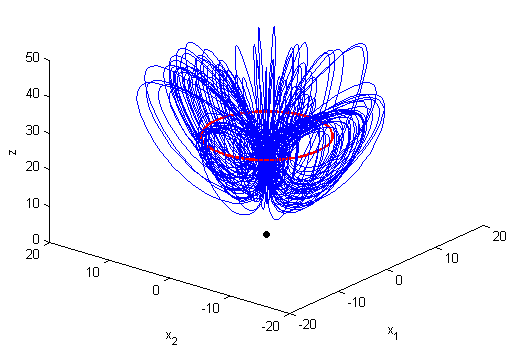
\includegraphics[width=0.35\textwidth]{Figs/Section2/kcCLEaxisonc.png}
b.)
  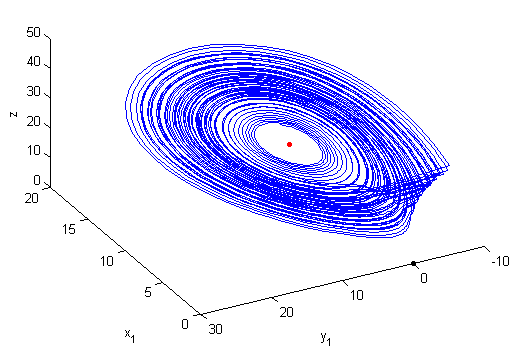
\includegraphics[width=0.35\textwidth]{Figs/Section2/kcCLEredaxisonc.png}
\caption{
a) A typical trajectory plotted in $(x_1, x_2, z)$ space.  Blue is the trajectory, the red is a travelling wave $TW_1$, and the black is the equilibrium at the origin.
b) Same trajectory as in part a, but this is symmetry reduced ($x_2 = 0$ space), and is plotted in $(x_1, y_1, z)$.  The trajectory no longer looks as messy as it was in part a.  The labelling is the same.
}
 \label{fig:CLETraj}
\end{figure}

A typical trajectory for the Complex Lorenz is seen in figure \ref{fig:CLETraj}a.  It is left to the reader to verify that the Complex Lorenz has $SO(2)$ symmetry, with the generator of the rotations given by \cite{CB}:
\[ \left( \begin{array}{ccccc}
0 & 1 & 0 & 0 & 0 \\
-1 & 0 & 0 & 0 & 0 \\
0 & 0 & 0 & 1 & 0\\
0 & 0 & -1 & 0 & 0 \\
0 & 0 & 0 & 0 & 0\end{array} \right)\]
Using equation \ref{eq:SymmGen}, we can compute a group element with phase $\phi$ as:
\begin{equation}
\left(
\begin{array}{ccccc}
\cos(\phi) & \sin(\phi) & 0 & 0 & 0 \\
-\sin(\phi) & \cos(\phi) & 0 & 0 & 0 \\
0 & 0 & \cos(\phi) & \sin(\phi) & 0\\
0 & 0 & -\sin(\phi) & \cos(\phi) & 0 \\
0 & 0 & 0 & 0 & 1
\end{array}\right)
\end{equation}
To find the relative equilibrium since we have $SO(2)$ symmetry, we switch over to polar coordinates $(r_1, r_2, \theta_1, \theta_2, z)$, and write the equations above as:
\begin{equation}
\begin{split}
  \dot r_1 &= -\sigma(r_1 - r_2\cos(\theta)) \\
  \dot r_2 &=   -r_2 + r_1((\rho_1 - z)\cos(\theta) - \rho_2\sin(\theta)) \\
  \dot \theta_1 &= -\sigma \frac{r_2}{r_1} \\
  \dot \theta_2 &= e + \frac{r_1}{r_2}((\rho_1 - z)\sin(\theta)+\rho\cos(\theta)) \\
  \dot z &= -bz  + r_1r_2\cos(\theta) \,,
    \label{eq:CLEpolar}
\end{split}
\end{equation}
where $r_1 = \sqrt{x_1^2 + x_2^2}$, $r_2 = \sqrt{y_1^2 + y_2^2}$, $\tan(\theta_1) = \frac{x_2}{x_1}$, $\tan(\theta_2) = \frac{y_2}{y_1}$, and $\theta = \theta_1-\theta_2$ \cite{CB}.

To have a relative equilibrium, we require: $\dot \theta_1 = \dot \theta_2$ and the remaining equations in \ref{eq:CLEpolar} to be set to $0$. It is left to the reader to verify that the equilibrium is given by:
\begin{equation}
(r_1, r_2, \theta, z) = (\sqrt{b(\rho_1-d)}, \sqrt{bd(\rho_1-d)}, \cos^{-1}(\frac{1}{\sqrt{d}}), \rho_1 - d)
\end{equation}
where $d = 1+ \frac{e^2}{(\sigma+1)^2}$.

(It should be noted that the constraint of $\dot \theta_1 = \dot \theta_2$ requires that $\sin(\theta) < 0$).  Using our parameters, a point on the relative equilibrium in $(x_1, x_2, y_1, y_2, z)$ coordinates is given by: $(8.4849,-0.0771,8.4885,0,26.9999$  \cite{CB}.
As mentioned, there are several ways to symmetry reduce this problem.  Here, we will post process into a slice, and unwisely choose our template and slice condition as:
\begin{equation}
\begin{split}
\hat{x} = (1, 0, 0, 0 , 0)\\
<\hat{x}'|t> = 0, t = \mathbf{T}\hat{x}
\label{eq:CLEslice}
\end{split}
\end{equation}
Using the slice condition (\ref{eq:SliceCond1}, \ref{eq:SliceCond2}) and the fact that we can write a point on the trajectory as $\hat{x}' = g^-1(\phi(t))x(t)$, we can compute the element $g \in G$ to meet our template and slice conditions \cite{SliceCond}.
With the knowledge of our relative equilibrium and a chosen slice, we a method to symmetry reduce our trajectory, and arrive at Figure \ref{fig:CLETraj}b.  We have reached the goals for this section: we have symmetry reduced a system.

Symmetries play an interesting role in dynamics.  When a system has a symmetry, there exists a set of solutions (we have called these relative equilibria) with trajectories in the same direction as the symmetry.  If these relative equilibria act as an attractor for a chaotic system, trajectories will tend to flow in the direction the relative equilibrium in addition to filling out the attractor \cite{Atl}.  As a result all of the interesting dynamics moves with the symmetries, and any hope of getting periodic orbits and relative periodic orbits is lost.  We could try to redefine the Poincar\'e section, but then the methods developed in the previous section would be for nothing.  With symmetry reduction, however, we remove all of these complications and we will only see the dynamics of interest; \cite{Atl} does an excellent job of explaining this in a nice analogy with drifters and dancers.

Having reviewed symmetries and how to reduce a symmetry, we now turn back to finding return maps, but we add an extra twist: the new system will have symmetry.

\section{Complex Lorenz Return Map}
\label{sec:CLE}
The obvious question is why symmetry reduction even necessary for finding a return map?  In short flows can be broken into two parts: (1) in the direction of the symmetry action, and (2) in directions orthogonal to the symmetry \cite{CB, Eth, Atl}.  The former complicates our goals of finding periodic orbits and relative periodic orbits; the latter is our concern, since imbedded in these are the relative equilibrium and relative periodic orbits \cite{Atl}.  When we symmetry reduce, the relative equilibrium become equilibrium and the relative periodic orbits become periodic orbits (periodic orbits, of course, will remain periodic orbits).  For a system without symmetry, we can find the periodic orbits; therefore, if we symmetry reduce a problem, we have \emph{reduced} the problem to a previously solved one.

Using Figure \ref{fig:CLETraj}, we see the relative equilibrium ($x_{TW}$) and the equilibrium ($x_0$, the origin) are the acting components to the attractor.  In analogy to the R\"ossler system, $x_{eq}^{-}$ is to $x_{eq}^{+}$ as $x_{TW}$ is to $x_0$.  Therefore, we want to look at how the unstable manifold originating from $x_{TW}$ unravels in a Poincar\'e section.
\begin{figure}[h]
\centering
a.)  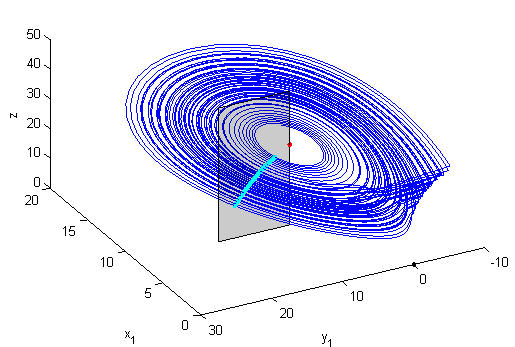
\includegraphics[width=0.35\textwidth]{Figs/Section3/kcCLEredaxisonPSc.png}
b.)
  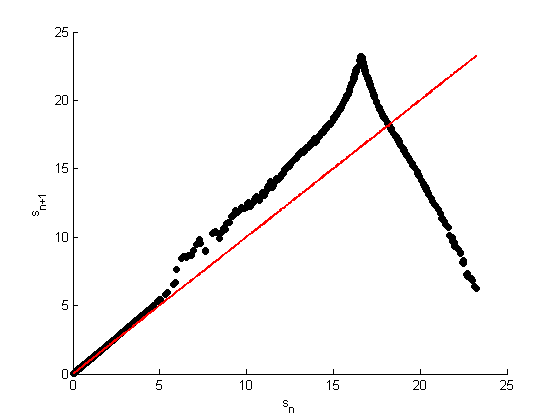
\includegraphics[width=0.35\textwidth]{Figs/Section3/kcCLEretmap.png}
\caption{ a) Reduced dynamics of the Complex Lorenz with a possible Poincar\'e section.  Usually, visualization of the Poincar\'e section is impossible since the symmetry reduced space is $4$-d, but we have used a simple section to help the reader. b) Return map for the complex Lorenz.  $s_n$ is the curvilinear distance.  This return map can be used to compute the relative periodic orbits seen in Figure \ref{fig:CLEPO}
}
 \label{fig:CLEretmap}
\end{figure}

Looking at a typical trajectory in reduced space (Figure \ref{fig:CLETraj}b), with the templates given by \ref{eq:CLEslice}, we can find a good Poincar\'e section will contain $x_{TW}$ and intersect all the interesting dynamics. For this particular example, we have chosen the section shown in \ref{fig:CLEretmap}a.  Following the same prescription as the R\"ossler system, we find the curvilinear distance along the curve of the unstable manifold in the Poincar\'e section and the return map.  The results are seen in Figure \ref{fig:CLEretmap}b.  A couple of relative periodic orbits in reduced space (appearing periodic) and in the original space are shown in Figure \ref{fig:CLEPO}.
 \begin{figure}
\centering
a.)  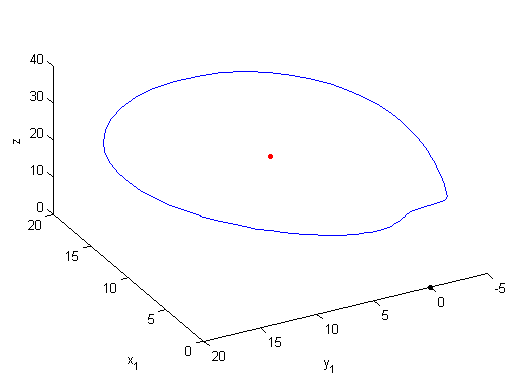
\includegraphics[width=0.35\textwidth]{Figs/Section3/kc1cyclec.png}
b.)
  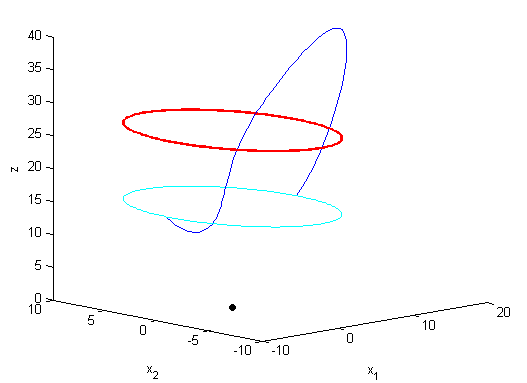
\includegraphics[width=0.35\textwidth]{Figs/Section3/kc1cycleunredc.png}
c.)
  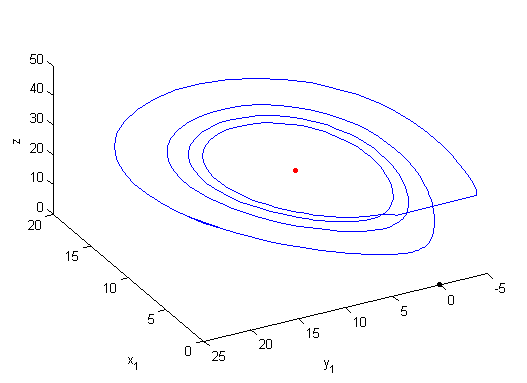
\includegraphics[width=0.35\textwidth]{Figs/Section3/kc4cyclec.png}
d.)
  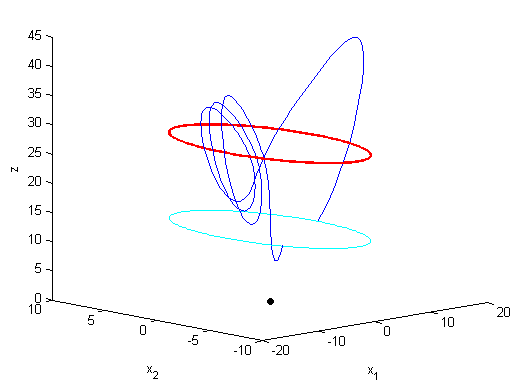
\includegraphics[width=0.35\textwidth]{Figs/Section3/kc4cyclewithcirclec.png}
\caption{Images depicted relative periodic orbits for the Complex Lorenz system.  The trajectories are in blue, the relative equilibrium red, and the equilibrium in black.
a) Cycle of length 1 for the Complex Lorenz system in reduced space (same template as Figure \ref{fig:CLETraj}. b) Same trajectory as part a, but plotted in unreduced space.  The group orbit of the initial point are shown in cyan; notice how the trajectory intersects this at the beginning and the end. c) Cycle of length $4$ for the Complex Lorenz in reduced space. d) Same cycle as part c, but in unreduced space; the group orbit of the starting and last point is given in cyan. }
 \label{fig:CLEPO}
\end{figure}

Summarizing, to find the (relative) periodic orbits of the Complex Lorenz, we followed the methods developed for the R\"ossler system with one extra step: we removed the symmetry of the Complex Lorenz.  The reasons for dividing out the symmetries were explained and with the reduced space, the relative periodic orbits of the Complex Lorenz were found.

The only difference between the Complex Lorenz and the R\"ossler system of equations were the added difficulty of the $SO(2)$ symmetry.  Removing symmetries for this case was easy, but in other cases, there will be problems.  Failures in symmetry reduction manifest themselves as discontinuities in dynamics \cite{Atl}.  For the Complex Lorenz, we avoided this problem, but it will rear its ugly head in other problems.  Methods for getting around these problems can be found in \cite{Atl}.

\section{Return Maps and Periodic Orbits}
\label{sec:Retmaps}
We have already discussed how a return map yields periodic orbits.  We demonstrated a few examples of the computed periodic solutions.  We turn now to a discussion of applications of return maps and periodic cycles to compute various entities of interest.  To expedite the process, we will assume the reader is familiar with the the concepts of entropy, transition graphs, and spectral determinants.  The reader unfamiliar with these topics can refer to \cite{CB}.  We will also focus on the R\"ossler system, so that we can compare our results.

For a return map, such as the one for the R\"ossler system, we will name any periodic orbit according to which regions it visits on a return map (Figure \ref{fig:Ross4cycle}a).  For example in Figure \ref{fig:Ross4cycle}, the periodic cycle $\overline{0111}$ starts in region $0$ iterates to region $1$ three times and then returns to $0$.  Using our return map, we can find the cycles of any order and have listed here the cycles up to order 7.  They are listed in Table below.

\begin{figure}[h]
\centering
a.)  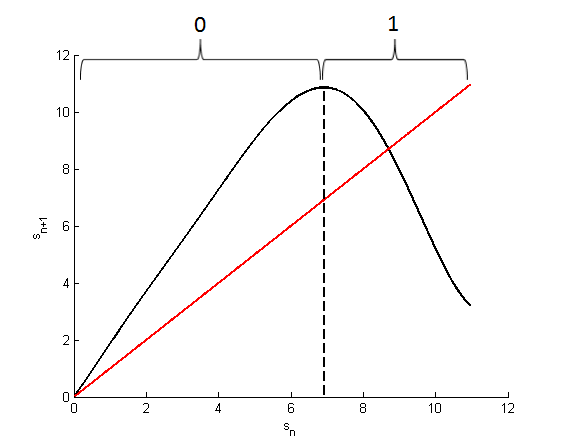
\includegraphics[width=0.35\textwidth]{Figs/Section4/kcdemon.png}
b.)  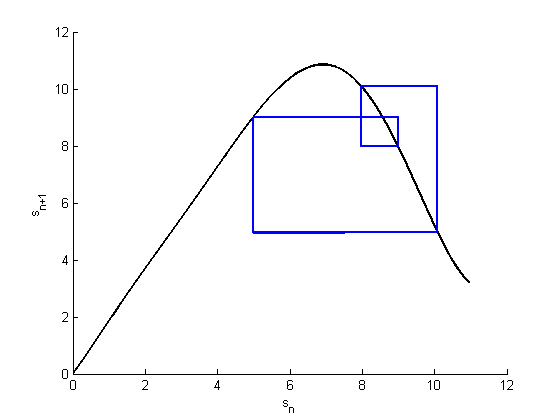
\includegraphics[width=0.35\textwidth]{Figs/Section4/kccycle4ross.png}
\caption{a) R\"ossler return map with symbolic dynamics defined.  Anything to the left of the critical point (marked with a dashed line) is labelled $0$, and anything to the right is labelled $1$. b) Cycles $\overline{0111}$ (blue) plotted on the R\"ossler return map.  Note that it start it $0$ iterates through region $1$ three times and then returns to its initial point.}
 \label{fig:Ross4cycle}
\end{figure}

\begin{center}
  \begin{tabular}{| l | c | c | c | c | c | c | c | c | r| }
    \hline
    $n_p$ & 1 & 2 & 3 & 4 & 5 & 6 & 7\\ \hline
    & $\overline{1}$ & $\overline{01}$ & $\overline{001}$ & $\overline{0111}$ & $\overline{01101}$ & $\overline{001011}$ & $\overline{0110101}$ \\
    &  &   & $\overline{011}$ &  & $\overline{01111}$ & $\overline{011101}$ & $\overline{0110111}$ \\
    &  &  &  &  &  & $\overline{011111}$ & $\overline{0111101}$ \\
    &  &  &  &  &  &  & $\overline{0111111}$ \\
    \hline
  \end{tabular}
\end{center}

For cycles up to length 5, we have also listed the leading Floquet multiplier (calculated from the Jacobian) and the periodicity of these trajectories in the table below.  These values can be compared with those computed in \cite{CB} and \cite{OtherRoss}.  Cycles of length $3$ and shorter compare well, beyond these lengths, however, they fail to agree; this could be due to computational limitations.

\begin{center}
  \begin{tabular}{| l | c | c | c  | r| }
    \hline
     & $\Lambda$ & $T_P$ \\ \hline
    $\overline{1}$  & -2.383 & 5.871\\ \hline
    $\overline{01}$ &  -3.618 & 11.780 \\ \hline
    $\overline{001}$ &  -2.318 & 17.492 \\ \hline
    $\overline{011}$ & 4.753 & 17.560  \\ \hline
    $\overline{0111}$ &  -17.532 & 23.544 \\ \hline
    $\overline{01101}$ &  -26.682 & 29.477 \\ \hline
    $\overline{01111}$ & 24.055 & 29.212 \\ \hline
  \end{tabular}
  \label{Tab:Eigenvales}
\end{center}

To find the entropy a system, we want to calculate the leading root of the polynomial:
\begin{equation}
\begin{split}
\text{det}|1-zT| &=0
\end{split}
\end{equation}
where $T$ is our transition matrix \cite{CB}. In theory this should be an infinite product, but for this work, we will truncate this to our 7th order.  We can reduce this polynomial to:
\begin{equation}
\begin{split}
\text{det}|1-zT| = 1 - t_{1}z - t_{01}z^2 - (t_{001} + t_{110} - t_{1}t_{01})z^3 \\ -(t_{0111} -t_{1}t_{001}-t_{1}t_{011})z^4  -(t_{01101}+t_{01111}-t_{01}t_{001}- \\ t_{01}t_{011}-t_{1}t_{0111})z^5 - \cdot \cdot \cdot
\end{split}
\end{equation}

\begin{equation}
\begin{split}
\text{det}|1-zT| &\approx 1 - z -z^2 - z^3 +z^4+z^5-z^6+z^7
\end{split}
\end{equation}

Calculation of the smallest root gives $z \approx .606684170874$.  The entropy $h = \text{ln}(z)$ is given by $h \approx -0.499746934907$.   This is the final result: we have demonstrated the use of return maps to calculate periodic orbits and calculated the entropy of the R\"ossler system, albeit we only did so up to order 7.

\section{Conclusion}
We have demonstrated the ability to compute periodic orbits for two systems.  The first system we examined was the R\"ossler attractor, and we developed a prescription to compute periodic orbits for chaotic systems through return maps.  In the second system, the Complex Lorenz, we were forced to deal with symmetries.  We showed that with symmetry reduction, we could reduce the problem from a complicated mess to a tractable problem: with symmetry reduced dynamics, we could now use our previous described methods and compute the return maps and several relative periodic orbits for the Complex Lorenz.  In the last section, we went over how the return maps could be used to compute entropy, and made an estimation for the entropy of the R\"ossler system.  The goals of this project were to find a return map for two systems, but along the way we learned how symmetries can cause difficulties.  Without symmetry reduction the difficulty of computing return maps and relative periodic orbits increases dramatically \cite{Eth}.  Symmetry reduction is crucial to solving problems, but \cite{Atl} points out that symmetry reduction may actually lead to some problems.  They have come up with a solution to deal with discontinuities that can arise in symmetry reduction, and while it would have been nice to try to implement those solutions here for computing return maps, a system with the appropriate parameters could not be found.  This is not without hope though and will continue to be investigated by this author.

\section{Acknowledgements}
The author would like to thank P. Cvitanovi\'c for his endless patience and many insightful conversations.  Without his input and direction, none of this would have been possible.

\begin{thebibliography}{9}

\bibitem{CB} P. Cvitanovi\'c, R. Artuso, R. Mainieri, G. Tanner, and G. Vattay, \emph{Chaos: Classical and Quantum} (Niels Bohr Inst. Copenhagen, 2011)
    chaosbook.org.

\bibitem{SRetMap} E. Siminos and P. Cvitanovi\'c, Physica D. {\bf 240}, 187 (2011).

\bibitem{Eth} E. Siminos \emph{Recurrent spatio-temporal structures in the presence of continuous symmetries}. PhD Thesis, School of Physics, Georgia Institute of Technology, Atlanta, 2009.
    ChaosBook.org/project/theses.html.

\bibitem{SliceCond} S. Froehlich and P. Cvitanovi\'c, Comm. Nonlinear Sci. and Numerical Simulation {\bf 17}, 2074 (2011).

\bibitem{Atl} P. Cvitanovi\'c, D. Borrero-Echeverry, K. Carroll, B. Robbins, E. Siminos, and L. Zhang. (2011 in prep)

\bibitem{OtherRoss} A. Basu, \emph{Construction of Poincar\'e return maps for R\"ossler flow}.
    ChaosBook.org/project


\end{thebibliography}
\end{document}
